%%%%%%%%%%%%%%%%%%%%%%%%%%%%%%%%%%%%%%%%%%%%%%%%%%%%%%%
% ultimate plantUML Cheatsheet
%   by Andreas Offenhaeuser
% Based on MatPlotLib Cheatsheet by Michelle Baltazar https://www.overleaf.com/latex/examples/matplotlib-and-random-cheat-sheet/yttxrcxntbht
%
%%%%%%%%%%%%%%%%%%%%%%%%%%%%%%%%%%%%%%%%%%%%%%%%%%%%%%%

\documentclass{article}
\usepackage[landscape]{geometry}
\usepackage[T1]{fontenc}
\usepackage{multicol}
\usepackage{scrextend}
\usepackage{amsfonts}
\usepackage[most]{tcolorbox}
\usepackage{tikz}
\usetikzlibrary{decorations.pathmorphing}
\usepackage{xcolor}

\usepackage{hyperref}
\hypersetup{
    colorlinks, breaklinks,
    linkcolor={red!50!black},
    citecolor={blue!50!black},
    urlcolor={blue!80!black}
}
\advance\topmargin-60pt
\advance\textheight3in
\advance\textwidth3in
\advance\oddsidemargin-110pt
\advance\evensidemargin-110pt
\parindent0pt
\parskip2pt

\newcommand{\block}[2]{%
  \begin{tikzpicture}%
  \node [draw=black, fill=white, very thick,
rectangle, rounded corners, inner sep=10pt, inner ysep=10pt] (box){%
    \begin{minipage}{0.3\textwidth}%
		#2%
    \end{minipage}%
  };%
\node[fill=black, text=white, font=\bfseries, right=10pt] at (box.north west) {#1};
\end{tikzpicture}%
}

\newcommand{\code}[1]{%
  \begin{tcolorbox}[frame hidden, interior hidden, grow to left by=-5pt,
  boxrule=0pt, boxsep=0pt, arc=0pt, breakable, before skip=4pt, after skip=5pt,]%
  \parbox{\textwidth}{\ttfamily\small #1}%
  \end{tcolorbox}
}

\title{ultimate PlantUML Cheatsheet}
\begin{document}
\begin{center}{\huge{\textbf{ultimate PlantUML Cheatsheet}}{\hspace*{40pt}\small v.COMMIT-ID}}\\
{\large by \href{http://anoff.io}{Andreas Offenhaeuser}}
\end{center}
\begin{multicols*}{3}

%%% COMPONENTS %%%
\block{Components}{
A list of plantUML components and their names, most can be used in any diagrams. The \textit{sequence} diagram only supports a subset.
  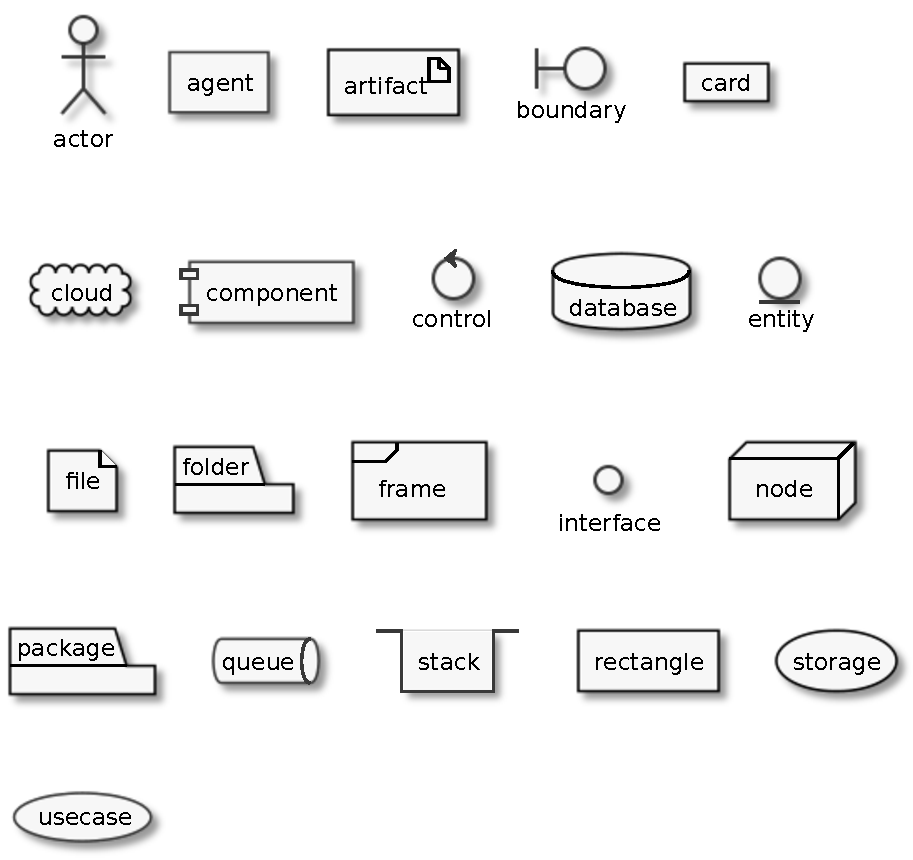
\includegraphics[width=\textwidth]{diagrams/dist/components.pdf} 
}

%%% SPRITE ICONS %%%
\block{Sprite icons}{
Additional icons can be added via sprites. There is a collection of \href{https://github.com/tupadr3/plantuml-icon-font-sprites}{Font Awesome, Developer, Government,.. icons} available via GitHub. Sprites can be included from any location that is reachable by the PlantUML server.

\code{
  !define ICONURL {\scriptsize https://raw.githubusercontent.com/\\
    tupadr3/plantuml-icon-font-sprites/v2.0.0} \\
  !includeurl ICONURL/common.puml \\
  !includeurl ICONURL/font-awesome-5/cogs.puml \\
  !includeurl ICONURL/govicons/submarine.puml \\

  FA5\_COGS(c1, work) \#white \\
  GOV\_SUBMARINE(sub1, Submarine1) \#lightblue \\
  GOV\_SUBMARINE(sub2, , frame, red) \{
  \begin{addmargin}[1em]{0em}
    FA5\_COGS(c2, more work, card, white) \#limegreen
  \end{addmargin}
  \}
}
\begin{center}
  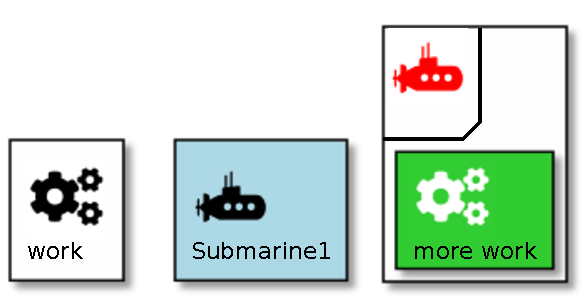
\includegraphics[height=70pt, width=0.9\textwidth, keepaspectratio]{diagrams/dist/icons-sprite.pdf}
\end{center}
}

%%% ICONS %%%
\block{Icons}{
PlantUML supports \href{https://useiconic.com/open/}{Open Iconic} set out of the box. Any icon can be rendered when embedding it in \textbf{<\&..>}.
\code{
card "<\&key> key"

card "<size:42><\&wrench></size>"
}
\begin{center}
  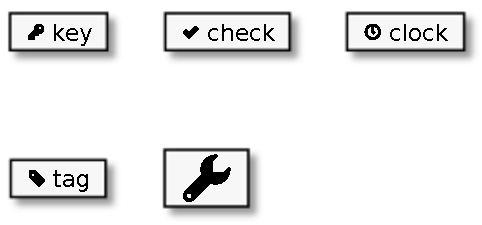
\includegraphics[height=70pt, width=0.45\textwidth, keepaspectratio]{diagrams/dist/icons.pdf}
  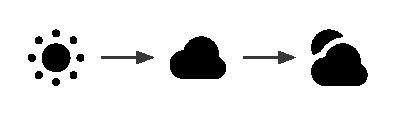
\includegraphics[height=70pt, width=0.45\textwidth, keepaspectratio]{diagrams/dist/icons-transparent.pdf}
\end{center}

Icons can be shown as icon only by disabling the border and background styles.

\code{
  rectangle "<size:150><\&sun></size>" as sun \\
  skinparam rectangleBorderColor none \\
  skinparam rectangleBackgroundColor none \\
  skinparam rectangleShadowing false
}
}

%%% MULTILINE %%%
\block{Multiline components}{
Text can be spread across multiple lines in components by declaring the text in \textbf{[ ]}.
\code{
node mynode [
\begin{addmargin}[1em]{0em}
    several \\
    lines \\
    ==== \\
    of \\
    .... \\
    text
\end{addmargin}
]
}
  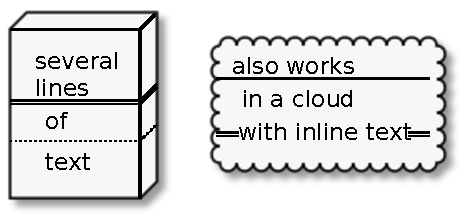
\includegraphics[width=0.7\textwidth]{diagrams/dist/multiline.pdf} 
}

%%% ARROWS %%%
\block{Arrows}{
PlantUML supports almost all \href{http://loufranco.com/wp-content/uploads/2012/11/cheatsheet.pdf}{UML arrow types}.
All combinations of two arrow heads and line type can be set.
\begin{center}
  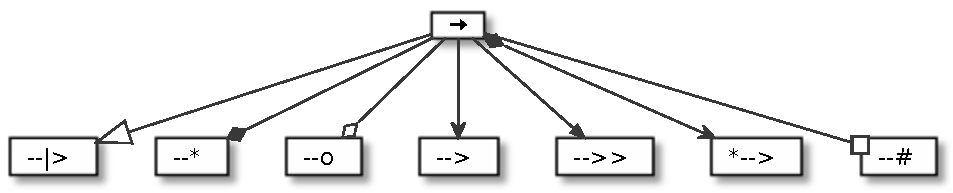
\includegraphics[height=80pt, width=0.9\textwidth, keepaspectratio]{diagrams/dist/arrows.pdf}

  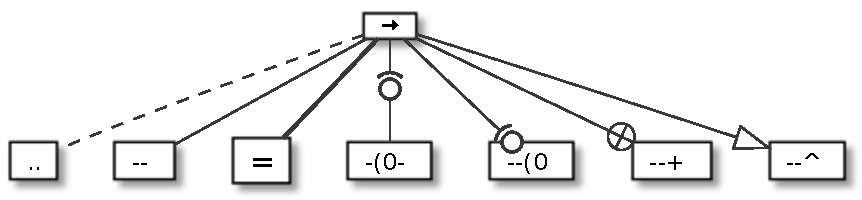
\includegraphics[height=80pt, width=0.9\textwidth, keepaspectratio]{diagrams/dist/arrows-2.pdf}
\end{center}
}

%%% SKINPARAM %%%
\block{Skinparam properties}{
For any \textit{component} style properties can be set via
\code{
skinparam <Component><Property> <value>
}

Multiple properties for the same component can be grouped
\code{
skinparam node \{
  \begin{addmargin}[1em]{0em}
  BackgroundColor transparent \\
  BorderColor black
  \end{addmargin}
\}
}

Component properties:

\textit{
  BackgroundColor, 
  BorderColor, 
  BorderThickness, 
  FontColor, 
  FontName, 
  FontSize, 
  FontStyle
}
\newline\newline
Generic properties:

\textit{
  ArrowColor, 
  ArrowLollipopColor, 
  ArrowThickness, 
  BackgroundColor, 
  DefaultTextAlignment {\small ([left], center, right)}, 
  Handwritten {\small [false]}, 
  HyperlinkColor, 
  HyperlinkUnderline, 
  Monochrome {\small [false]}, 
  Nodesep {\small (horizontal margin [0])}, 
  Padding {\small (text padding within node [0])}, 
  Ranksep {\small (vertical margin [0])}, 
  RoundCorner, 
  Shadowing
}
\newline\newline
The full list of \href{http://plantuml.com/skinparam}{skinparam settings} and \href{http://plantuml.com/color}{available colors} can be found on the \href{http://plantuml.com/}{plantUML website}.
}

\block{Component diagrams}{
  Enforcing layout..
}
\block{Useful links}{
  \begin{itemize}
  \item \href{http://plantuml.com/color}{Available colors}
  \item \href{http://plantuml.com/skinparam}{Stylable properties}
\end{itemize}
}

\end{multicols*}
\end{document}